\documentclass{llncs2e/llncs}

\usepackage{graphicx}
\usepackage{amssymb}
\usepackage{amsmath}
\usepackage{listings}
\usepackage{pgf,tikz}
\usepackage{algorithm}
\usepackage{algpseudocode}
\usepackage{wrapfig}
\usetikzlibrary{positioning}

\begin{document}
\setcounter{page}{0}
\pagestyle{headings}
\title{Defining and Model-Checking an Epistemic Temporal Logic with Changes of Observations}
\titlerunning{CTL$^{*}$K$\Delta$}
\author{Aur\`ele Barri\`ere}
\authorrunning{Aur\`ele Barri\`ere}
\date{December 18, 2017}
\institute{\'Ecole Normale Sup\'erieure de Rennes, France\\
\email{aurele.barriere@ens-rennes.fr}\\
}
\maketitle
\hrulefill
\begin{center}
  \textbf{Supervisors: }\\
  Aniello Murano\\
  Bastien Maubert\\
  Sasha Rubin\\
  ~\\
  Universit\`a degli Studi di Napoli Federico II
\end{center}
\hrulefill
\begin{center}
  \textbf{September 11th, 2017 - December 11th, 2017}
\end{center}
\vfill
\begin{abstract}  
We define a logic for systems with imperfect information, CTL$^*$K$\Delta$. It inherits operators from temporal and epistemic logics, as well as a new one that allows agents to dynamically change their observation of the system. We first define it for single-agent settings with synchronous perfect recall. We define an equivalent semantics, that is used later for model-checking the logic, and proved to be equivalent. We give an algorithm for model-checking. Finally, we extend our logic to multi-agent settings.
\keywords{Epistemic Temporal Logic, Model Checking, Changing Observations}
\end{abstract}
\vfill
\newpage

% macros
\def\ctls{CTL$^{*}$}
\def\ctlskd{CTL$^{*}$K$\Delta$}
\def\ctlskdp{CTL$^{*}$K$\Delta\psi$}
\def\ap{AP}
\def\A{\mathit{A}}
\def\E{\mathit{E}}
\def\U{\mathit{U}}
\def\R{\mathit{R}}
\def\X{\mathit{X}}
\def\K{\mathit{K}}
\def\KP{\bar{\mathit{K}}}
\def\D#1{\Delta^{#1}}
\def\eq#1#2{\approx^{#2}_{#1}}
\def\eqh#1{\approx_{#1}}
\def\eqstate#1{\sim_{#1}}
\def\todo#1{{\color{red}#1}}
\def\iff{\ \mathit{iff}\ }
\def\UD{U_{\Delta}}
\def\UT{U_T}
\def\UDK#1{U_{\Delta #1}}
\def\UTK#1{U_{T #1}}
\def\FV{\mathit{FH}}
\def\FP{\mathit{FP}}
\def\ktree{$k$-tree}
\def\ktrees{$k$-trees}
\def\qed{\hfill$\blacksquare$}

\section{Introduction}
\label{sec:intro}
Epistemic Logics are well known to be a required formalism to describe and reason about knowledge in distributed systems. Distributed algorithms (also called \textit{protocols}) involve agents without complete knowledge of the state of the system. Therefore, ``Any logic of protocols must include as part of it a logic of knowledge'', as said by Ladner and Reif in~\cite{DBLP:conf/tark/LadnerR86}.
Such systems have been found to be useful for in many areas, including Game Theory and Artificial Intelligence.
A popular extension of Epistemic Logics is to combine them with Temporal Logics. Reasoning about the evolution of agents' knowledge inside a system becomes possible. For each of these logics, model-checking (deciding if a formula is true in a given model) is an important problem, as it allows to confront the model of a system to its specification.

In these settings, agents are usually given a fixed observation for the whole evolution. Observations describe an agent's point of view, to model imperfect information.
In this paper, to deal with dynamic changes of observations during the evolution in a system with imperfect information, we introduce a new logic, \ctlskd. To the best of our knowledge, this is the first time that such changes are studied. This logic includes branching-time temporal operators, epistemic operators, and a new one, $\D{o}$, to represent changes of observation. For instance, the formula $\D{o}\K\A\X p$ states that after changing to an observation $o$, the agent knows that, on the next step, the proposition $p$ holds.


This logic could be useful for any system where agents can change their observational power of the system. For instance, in a scenario where there exists different ``security levels'' where different levels have access to different information. With our logic, it becomes possible to express statements such as ``For an agent with initial observation $o_1$, there exists a point in time where, if the agent changes his observation to $o_2$, he knows whether or not some proposition holds'' ($\D{o_1}F(\D{o_2}(\K p\vee\K\neg p))$).
Another main motivation to define such a logic is the work that has been done on Strategy Logic with Imperfect Information~\cite{DBLP:conf/lics/BerthonMMRV17}, an extension of Strategy Logic~\cite{DBLP:journals/iandc/ChatterjeeHP10}. In this logic, agents can change observation when changing strategies.
Before investigating it in the full framework of Strategy Logic, the natural first step was to study the interactions of observation changes, knowledge and time in a simpler setting, without the strategic aspects.

In Section~\ref{sec:ctlskd}, we first define the logic \ctlskd. To begin, we only define it for single-agent synchronous perfect recall settings.
Then, in Section~\ref{sec:alternative}, we introduce an alternative, finitary semantics for the same formulas, that we later prove to be equivalent to the first one, and easier to model-check.
In Section~\ref{sec:mc}, we describe an algorithm to model-check a formula of \ctlskd.
Finally, we extend the logic for multi-agent settings in Section~\ref{sec:multi}.


\subsubsection{Related Works}
Works on epistemic logics are numerous. The first ones started to investigate logics of knowledge in a static setting~\cite{sato77}. Later, many works have studied combinations of epistemic and temporal logics. Such logics are said to be Epistemic Temporal Logics~\cite{Dima2009}.

In~\cite{DBLP:conf/fsttcs/MeydenS99}, the logic LTLK is defined and model-checked. We use the same \ktree\ structure in Section~\ref{sec:multi} to represent the knowledge of multiple agents.

Without our changes of observations, the combination of CTL with epistemic logics has been studied before~\cite{DBLP:conf/birthday/LomuscioP12}\cite{DBLP:conf/faabs/LomuscioLP02}.
CTL$^*$, the extension of CTL, has also been studied with epistemic operators. CTL$^*$K has been investigated and model-checked in~\cite{DBLP:conf/atal/KongL17}\cite{DBLP:phd/hal/Maubert14}\cite{BOZZELLI201580}, in both memoryless and perfect recall settings.


The possibility of dynamically changing observation has been introduced in Strategy Logic with Imperfect Information~\cite{DBLP:conf/lics/BerthonMMRV17}. In this logic, an operator $(a,x)$ allows to assign a strategy $x$ to a player $a$. Strategies are defined with the operator $\ll x\gg^o$, where $o$ is an observation, because strategies for imperfect information systems can only be defined with regards to some observation. Whenever a strategy is assigned to a player, this player will behave as if he sees the system with the observation that his strategy was defined with. In that sense, it is possible for a player to change his observation power if he changes his strategy to another one using a different observation. A natural extension to Strategy Logic with imperfect information being epistemic operators, we decided to study how such changes of observation would interact with the agents' knowledge, by defining a dedicated operator.




\section{\ctlskd}
\label{sec:ctlskd}
\begin{frame}{\ctlskd\quad Syntax}

  \begin{block}{Syntax}
    \begin{tabular}{r l}
    History Formula: & $\varphi := p ~|~ \neg \varphi ~|~ \varphi\wedge\varphi ~|~ \A\psi ~|~$\color{red!85!blue}$ \K\varphi ~|~ \D{o}\varphi$\\
    Path Formula: & $\psi := \varphi ~|~ \neg\psi ~|~ \psi\wedge\psi ~|~ \X\psi ~|~ \psi\U\psi$
    \end{tabular}
  \end{block}
  \vfill
  \begin{block}{Definitions}
    History: finite sequence of states.\\
    Path: infinite sequence of states.
  \end{block}
  
\end{frame}


\begin{frame}{\ctlskd\quad Models}

  \begin{block}{Kripke Structures with Observations}
    $AP$ atomic propositions.
    $\mathcal{O}$ set of $m$ observations.

    $M=(S,I_s,o_I,T,V,\eqstate{o_1},\dots,\eqstate{o_m})$ where:

    \begin{tabular}{r l}
      $S$& set of states.\\
      $I_s\subseteq S$& set of initial states.\\
      \color{red!85!blue}$o_I$& initial observation.\\
      $T\subseteq S\times S$& transition relation.\\
      $V:S\rightarrow 2^{\mathit{AP}}$& valuation function.\\
      \color{red!85!blue}$\forall o_i, \eqstate{o_i}$& equivalence relations between states (observation).
    \end{tabular}
  \end{block}
  
\end{frame}


\begin{frame}{Defining \ctlskd\ Semantics}

  \begin{block}{Observation records}
    To get possible histories, we need to remember the previous states and corresponding observations.\\
    $r=[(o_1,0),(o_2,3),(o_3,3)]$.
    Agent had observations
    \begin{tabular}{l l}
      $o_I$ and $o_1$ & at time 0\\
      $o_1$ & at time 1 and 2\\
      $o_1,o_2$ and $o_3$ & at time 3\\
      $o_3$ & at time 4 and more.
    \end{tabular}
  \end{block}
  \vfill
  \begin{block}{Equivalent histories}
    $h\eqh{r}h'\quad\iff\quad \forall i< |h|, \forall o$ observation at time $i$ according to $r$, $h(i)\eqstate{o} h'(i)~\textit{and}~|h|=|h'|.$
  \end{block}
  
\end{frame}


\begin{frame}{\ctlskd\quad Semantics}
  \footnotesize
  \begin{block}{Semantics}
    \begin{tabular}{l c l}
      $M,h,r \models p $&$ \iff $&$ p\in V(\mathit{last}(h))$\\
      $M,h,r \models \neg\varphi $&$ \iff $&$ M,h,r\not\models\varphi$\\
      $M,h,r \models \varphi_1\wedge\varphi_2 $&$ \iff $&$ (M,h,r\models\varphi_1~\text{and}~ M,h,r\models\varphi_2)$\\
      $M,h,r \models \A\psi  $&$ \iff $&$ \forall\pi$ that extends $h$, we have $M,\pi,|h|-1,r\models\psi$\\
      \color{red!85!blue}$M,h,r \models\K\varphi  $&$ \iff $&\color{red!85!blue}$ \forall h'$ such that $h'\eqh{r}h$, we have $M,h',r\models\varphi$\\
      \color{red!85!blue}$M,h,r \models \D{o}\varphi $&$ \iff $&\color{red!85!blue}$ M,h,r[(o,|h|-1)]\models\varphi$\\
      $M,\pi,n,r\models\varphi $&$ \iff $&$ M,(\pi_0\dots\pi_n),r\models\varphi$\\
      $M,\pi,n,r\models\neg\psi $&$ \iff $&$ M,\pi,n,r\not\models\psi$\\
      $M,\pi,n,r\models \psi_1\wedge\psi_2 $&$ \iff $&$ (M,\pi,r,n\models\psi_1~\text{and}~ M,\pi,r,n\models\psi_2)$\\
      $M,\pi,n,r\models\X\psi $&$ \iff $&$  M,\pi,(n+1),r\models\psi$\\
      $M,\pi,n,r\models \psi_1\U\psi_2 $&$ \iff $&$ \exists m\geq n$ such that $\forall k\in[n,m[, M,\pi,k,r\models\psi_1$\\
          & & and $M,\pi,m,r\models\psi_2$
    \end{tabular}
  \end{block}
\end{frame}

\begin{frame}{A few validities of \ctlskd}

  \begin{block}{Truth}
    $\K\varphi\quad\rightarrow\quad\varphi$
  \end{block}
  \vfill
  \begin{block}{Distributivity}
    $\D{o}(\varphi_1\wedge\varphi_2)\quad\leftrightarrow\quad(\D{o}\varphi_1\wedge\D{o}\varphi_2)$
  \end{block}
  \vfill
  \begin{block}{Self-Duality}
    $\D{o}\neg\varphi\quad\leftrightarrow\quad\neg\D{o}\varphi$
  \end{block}
  \vfill
  \begin{block}{Redundant change of observation}
    $\D{o}\A\X\D{o}\K\varphi\quad\leftrightarrow\quad\D{o}\A\X\K\varphi$
  \end{block}
\end{frame}


\begin{frame}{Model Checking \ctlskd}

  \begin{block}{Marking Algorithm}
    Inductively mark the states of the model where each subformula holds.
  \end{block}
  \vfill
  \begin{alertblock}{The current semantics can't be model-checked this way}
  \end{alertblock}
  \vfill
  \begin{exampleblock}{Define Alternative Semantics}
    \begin{itemize}
    \item Extract information from histories and records.
    \item Model-Check the new Semantics.
    \item Prove that the two semantics are equivalent.
    \end{itemize}
  \end{exampleblock}
  
\end{frame}


\section{Alternative Semantics}
\label{sec:alternative}
We now introduce another semantics to interpret formulas of \ctlskd.
In this semantics, we aim to replace histories and observation records with information sets (intuitively, the set of states the agent believe it is possible to be in). 

\subsection{Information sets}
In this semantics, history formulas are interpreted on $s$ a state of the model, $I$ an information set (set of model states) and $o$ the current observation.
Path formulas are interpreted on $\pi$ an infinite sequence of states of the model starting in the current one (we don't remember the past states), $I$ the information set and $o$ the current observation.

%Later in this section, we will prove an equivalence between the two semantics for \ctlskd. If the first semantics corresponds to the intuitive semantics that we want to model-check, this new semantics offer some advantages. First, the past history is forgotten, for history and path formulas. We show that the information set captures enough information about the past. Secondly, because there exists a finite number of information sets, this new semantics is easier to model-check.

\paragraph{Preliminary definitions}
If $\pi=\pi_0\pi_1\dots$ is an infinite sequence of states, we write $\pi_{n\dots}$ the infinite sequence $\pi_n\pi_{n+1}\dots$.

We define two functions to update information sets. $\UD$ updates the set when a player goes through a change of observation and $\UT$ updates the set when the player moves to a new state. 
Finally, we define a function $I_I$ to get the initial information set from an initial state and an initial observation.

\begin{tabular}{r c c c l}
$\UD(I,s,o)$& = &$\{x\in I$ & $~|~$ & $x\eqstate{o}s\}$\\
$\UT(I,s,o)$& = &$\{x\in S$ & $~|~$ & $\exists t\in I, t\rightarrow x ~\text{and}~ x\eqstate{o}s\}$\\
$I_I(s_I,o_I)$& = &$\{s\in S$ & $~|~$ & $s\eqstate{o_I}s_I\}$\\
\end{tabular}

When we are in state $s$ with information set $I$ and the observation changes to $o$, the new information set is $\UD(I,s,o)$.
When we move to a new state $s$ with information set $I$ and observation $o$, the new information set is $\UT(I,s,o)$

For a path $\pi$ and $n\in\mathbb{N}$, we write $\UT^n(I,\pi,o)$ the successive temporal updates from $\pi_0$ to $\pi_n$.

$\UT^0(I,\pi,o)=I$\quad and\quad$\UT^{n+1}(I,\pi,o)=\UT(\UT^n(I,\pi,o),\pi_{n+1},o)$

\subsection{Information Set Semantics}~

\begin{tabular}{l c l}
  $M,s,I,o\models p $&$ \iff $&$ p\in V(s)$\\
  $M,s,I,o\models\neg\varphi $&$ \iff $&$ M,s,I,o\not\models\varphi$\\
  $M,s,I,o\models \varphi_1\wedge\varphi_2 $&$ \iff $&$ (M,s,I,o\models\varphi_1~\text{and}~M,s,I,o\models\varphi_2)$\\
  $M,s,I,o\models\A\psi $&$ \iff $&$ \forall\pi$ such that $\pi_0=s$, we have $M,\pi,I,o\models\psi$\\
  $M,s,I,o\models\K\varphi $&$ \iff $&$ \forall s'\in I$, we have $M,s',I,o\models\varphi$\\
  $M,s,I,o'\models\D{o}\varphi $&$ \iff $&$ M,s,\UD(I,s,o),o\models\varphi$\\
  $M,\pi,I,o\models\varphi $&$ \iff $&$ M,\pi_0,I,o\models\varphi$\\
  $M,\pi,I,o\models\neg\psi $&$ \iff $&$ M,\pi,I,o\not\models\psi$\\
  $M,\pi,I,o\models\psi_1\wedge\psi_2 $&$ \iff $&$ (M,\pi,I,o\models\psi_1~\text{and}~M,\pi,I,o\models\psi_2)$\\
  $M,\pi,I,o\models\X\psi $&$ \iff $&$ M,\pi_{1\dots},\UT(I,\pi_1,o),o\models\psi$\\
  $M,\pi,I,o\models\psi_1\U\psi_2 $&$ \iff $&$ \exists n\geq 0$, $\forall m\leq n, M,\pi_{m\dots},\UT^m(I,\pi,o),o\models\psi_1$ and\\
   & & $M,\pi_{n\dots},\UT^n(I,\pi,o),o\models\psi_2$
\end{tabular}

\subsection{Reduction Theorem}
We now have different semantics, that share the same syntax. We will now prove that these two semantics are equivalent.

To do so, we first notice that, from a history $h$ and an observation record $r$, we can get corresponding current state, information set and current observation. Similarly, from an infinite sequence $\pi$, a time $n$ and a record, we can get corresponding sequence $\pi'$ that starts at the current state, information set and current observation.

We accordingly define two partial functions, $\FV$ and $\FP$ as follows:

\paragraph{$\FV(h,r)=(s,I,o)$} where

\begin{tabular}{r l}
\textsc{i)} & \quad$s=\mathit{last}(h)$\\
\textsc{ii)} & \quad$o=\mathit{last}(r_{\leq |h|-1})$\\
\textsc{iii)} & \quad$I=f(h,r)$
\end{tabular}

\paragraph{$\FP(\pi,n,r)=(\pi',I,o)$} where

\begin{tabular}{r l}
\textsc{iv)} & \quad$\pi'=\pi_{n\dots}$\\
\textsc{v)} & \quad$o=\mathit{last}(r_{\leq n})$\\
\textsc{vi)} & \quad$I=f((\pi_0,\dots,\pi_n),r)$
\end{tabular}

$\FV$ and $\FP$ are partial functions, because
$\FV(h,r)$ is defined only if $r=r_{\leq |h|-1}$
and $\FP(\pi,n,r)$ is defined only if $r=r_{\leq n}$.

\paragraph{$f$} is defined inductively as follows: ($s$ is a state, $h$ a history)

\begin{tabular}{r c l}
$f(s,r)$&$=$&$I_I(s,o_I)~\text{if $r_0$ is empty}$\\
$f(s,r)$&$=$&$\UD(\UD(\dots\UD(I_I(s,o_I),s,o_1),s,o_2)\dots,s,o_m)~\text{if $r_0=[o_1,o_2,\dots,o_m]$}$\\
$f(h.s,r)$&$=$&$\UT(f(h,r),s,\mathit{last}(r_{\leq |h|-1}))~\text{if $r_{|h|}$ is empty}$\\
$f(h.s,r)$&$=$&$\UD(\dots\UD(\UT(f(h,r),s,\mathit{last}(r_{\leq |h|-1})),s,o_1)\dots,s,o_m)~\text{if $r_{|h|}=[o_1,\dots,o_m]$}$
\end{tabular}

\subsubsection{Lemmas}~

\textbf{Information Set Lemma} If $f(h,r)=I$, then\\
$I=\{s\in S~|~\exists h',h'\eqh{r}h~\text{and}~\mathit{last}(h')=s\}.$

\textbf{Proof:} This is proved inductively.
\begin{itemize}
\item Let $s\in S$ and $r$ a record. If $r_0$ is empty, then $\{s'\in S~|~\exists h',h'\eqh{r}s~\text{and}~\mathit{last}(h')=s'\}=\{s'\in S~|~s'\eqstate{o_I}s\}=I_I(s,o_I)$. This is the definition of $f(s,r)$.
\item If $r_0=[o_1\dots o_m]$, then $\{s'\in S~|~\exists h',h'\eqh{r}s~\text{and}~\mathit{last}(h')=s'\}=\{s'\in S~|~s'\eqstate{o_i}s,\forall o_i\in r_0\cup\{o_I\}\}$. This is the definition of $f(s,r)$.
\item Let $h$ be a history and $r$ a record. Let $o_r=\mathit{last}(r_{\leq |h|-1})$. If $r_{|h|}$ is empty\\
$\{s'\in S~|~\exists h',h'\eqh{r}h.s~\text{and}~\mathit{last}(h')=s'\}$\\
$=\{s'~|~\exists h', h'\eqh{r}h, \mathit{last}(h')\rightarrow s' ~\text{and}~s'\eqstate{o_r}s\}$\\
$=\{s'~|~\exists t\in f(h,r), t\rightarrow s'~\text{and}~s'\eqstate{o_r}s\}$ by induction hypothesis\\
$=\UT(f(h,r),s,o_r)$.
\item Let $o_r=\mathit{last}(r_{\leq |h|-1})$. If $r_{|h|}=[o_1\dots o_m]$, then\\
$\{s'\in S~|~\exists h',h'\eqh{r}h.s~\text{and}~\mathit{last}(h')=s'\}$\\
$=\{s'~|~\exists h', h'\eqh{r}h, \mathit{last}(h')\rightarrow s' ~\text{and}~s'\eqstate{o}s\forall o\in [o_1\dots o_m]\cup\{o_r\}\}$\\
$=\{s'~|~\exists t\in f(h,r), t\rightarrow s'~\text{and}~s'\eqstate{o}s\forall o\in [o_1\dots o_m]\cup\{o_r\}\}$ by induction hypothesis\\
$=\UD(\dots\UD(\UT(f(h,r),s,o_r),s,o_1)\dots,s,o_m)$.\qed
\end{itemize}

We now present useful results about the functions $\FV$ and $\FP$. The proofs of the following lemmas can be found in appendix, Section~\ref{subsec:lemmaproof}.

\textbf{Lemma 1}
Let $h,h'$ and $r$ such that $h\eqh{r}h'$. Let $(s,I,o)=\FV(h,r)$ and $(s',I',o')=\FV(h',r)$. We have $I=I'$ and $o=o'$.

\textbf{Lemma 2}
Let $(s,I,o)=\FV(h,r)$.\\ Then, $\forall\pi$ such that $\pi_0=s$, $\FP(h.\pi_{1\dots},|h|-1,r)=(\pi,I,o)$.

\textbf{Lemma 3}
Let $(s,I,o)=\FV(h,r)$. Then, $\FV(h,r[(o',|h|-1)])=(s,\UD(I,s,o'),o')$.

\textbf{Lemma 4}
Let $(\pi',I,o)=\FP(\pi,n,r)$. Then, $\FV(\pi_0\dots\pi_n,r)=(\pi'_0,I,o)$.

\textbf{Lemma 5}
Let $(\pi',I,o)=\FP(\pi,n,r)$. Then, $\FP(\pi,n+1,r)=(\pi'_{1\dots},\UT(I,\pi'_1,o),o)$.

\textbf{Lemma 6}
Let $(\pi',I,o)=\FP(\pi,n,r)$.\\ Then, $\forall k\geq 0, \FP(\pi,n+k,r)=(\pi'_{k\dots},\UT^k(I,\pi',o),o)$.

\subsubsection{Reduction Theorem}
$\forall\phi$ formula of \ctlskd,\\
if $\phi=\varphi$ is a history formula, $\forall h,r,s,I,o$ such that $\FV(h,r)=(s,I,o)$,\\ $M,h,r\models\varphi\iff M,s,I,o\models\varphi$,\\
if $\phi=\psi$ is a path formula, $\forall \pi,n,r,\pi',I,o$ such that $\FP(\pi,n,r)=(\pi',I,o)$,\\ $M,\pi,n,r\models\psi\iff M,\pi',I,o\models\psi$.

\textbf{Proof} By induction on $\phi$.
Let $h,r,s,I,o$ such that $\FV(h,r)=(s,I,o)$.
For each case, we prove \textbf{1:} if $M,h,r\models\varphi$ then $M,s,I,o\models\varphi$,
and \textbf{2:} if $M,s,I,o\models\varphi$ then $M,h,r\models\varphi$,
\begin{itemize}
\item\underline{$p$~\textbf{1: and 2:}} We have $p\in V(\mathit{last}(h))\iff p\in V(s)$, because $\FV(h,r)=(s,I,o)$. Thus, $M,h,r\models p\iff M,s,I,o\models p$.
\item\underline{$\neg\varphi$~\textbf{1: and 2:}} We have $M,h,r\not\models\varphi\iff M,s,I,o\not\models\varphi$ by induction hypothesis.
\item\underline{$\varphi_1\wedge\varphi_2$~\textbf{1 and 2:}} We have $M,h,r\models\varphi_1~\text{and}~M,h,r\models\varphi_2\iff M,s,I,o\models\varphi_1~\text{and}~M,s,I,o\models\varphi_2$ by induction hypothesis.
\item\underline{$\A\psi$~\textbf{1:}} We have $\forall\pi'$ extending $h$, $M,\pi',|h|-1,r\models\psi$. Let $\pi$ such that $\pi_0=s$. Let us prove that $M,\pi,I,o\models\psi$.
We have $\FP(h.\pi_{1\dots},|h|-1,r)=(\pi,I,o)$, because $\FV(h,r)=(s,I,o)$ (\textbf{Lemma 2}). Then by induction, because $h.\pi_{1\dots}$ extends $h$ and $ M,h.\pi_{1\dots},|h|-1,r\models\psi$, we have $M,\pi,I,o\models\psi$.
\item\underline{$\A\psi$~\textbf{2:}} Assume $\forall\pi'$ such that $\pi'_0=s$, $M,\pi',I,o\models\psi$. Let $\pi$ an infinite sequence of states. Let us prove that $M,h.\pi,|h|-1,r\models\psi$. By induction, it suffices to prove that $M,s.\pi,I,o\models\psi$, because $\FP(h.\pi,|h|-1,r)=(s.\pi,I,o)$ (\textbf{Lemma 2}). $s.\pi$ is a run $\pi'$ such that $\pi'_0=s$, and thus $M,h,r\models\A\psi$.
\item\underline{$\K\varphi$~\textbf{1:}} Assume that $\forall h_1\eqh{r}h, M,h_1,r\models\varphi$. Let $s'\in I$. Let us prove that $M,s',I,o\models\varphi$. Using the \textbf{Information Set Lemma}, there exists some $h_1\eqh{r}h$ with $\mathit{last}(h_1)=s'$. We then have $\FV(h_1,r)=(s',I,o)$ (\textbf{Lemma 1}). As $M,h_1,r\models\varphi$, we conclude by induction that $M,s',I,o\models\varphi$ and thus $M,s,I,o\models\K\varphi$.
\item\underline{$\K\varphi$~\textbf{2:}} Assume that $\forall s'\in I, M,s',I,o\models\varphi$. Let $h'$ such that $h'\eqh{r}h$. Let $s'=\mathit{last}(h')$. We have that $\FV(h',r)=(s',I,o)$ (\textbf{Lemma 1}). Because $s'\in I$ (\textbf{Information Set Lemma}), by induction we conclude $M,h',r\models\varphi$, and then $M,h,r\models\K\phi$.
\item\underline{$\D{o'}\varphi$~\textbf{1: and 2:}} Using \textbf{Lemma 3}, we have $\FV(h,r[(o',|h|-1)])=(s,\UD(I,s,o'),o')$.
Then, by induction, $M,h,r[(o',|h|-1)]\models\varphi\iff M,s,\UD(I,s,o'),o'\models\varphi$.
\end{itemize}
Let $\pi,n,r,\pi',I,o$ such that $\FP(\pi,n,r)=(\pi',I,o)$.
\begin{itemize}
\item\underline{$\varphi$} With \textbf{Lemma 4}, we have $\FV(\pi_0\dots\pi_n,r)=(\pi'_0,I,o)$ and thus by induction, $M,\pi_0\dots\pi_n,r\models\varphi\iff M,\pi'_0,I,o\models\varphi$. Finally, $M,\pi,n,r\models\varphi\iff M,\pi',I,o\models\varphi$.
\item\underline{$\neg\psi$ and $\psi_1\wedge\psi_2$} Apply the induction hypothesis.
\item\underline{$\X\psi$} With \textbf{Lemma 5}, we have $\FP(\pi,n+1,r_{\leq n})=(\pi'_{1\dots},\UT(\pi'_1,I,o),o)$ and thus by induction,
$M,\pi,n,r\models\X\psi\iff M,\pi',I,o\models\X\psi$.
\item\underline{$\psi_1\U\psi_2$} According to the definitions, it suffices to prove that $\forall k\geq 0$ and $\psi$ subformula of $\psi_1\U\psi_2$,
$M,\pi'_k,\UT^k(I,\pi',o)\models\psi\iff M,\pi,n+k,r\models\psi$. This result comes from the induction hypothesis and \textbf{Lemma 6}.\qed
\end{itemize}


\section{Model-Checking \ctlskd}
\label{sec:mc}
\subsubsection{Model-Checking problem} Given a model $M=(S,I_s,o_I,T,V,\eqstate{o_1},\dots,\eqstate{o_m})$ and a history formula $\varphi$, return \textbf{yes} if $M\models\varphi$, and \textbf{no} otherwise.
Thanks to the reduction theorem, it suffices to show that, for each $s\in I_s$, $M,s,I_I(s,o_I),o_I\models\varphi$. The algorithm will check the formula according to the information set semantics.

\subsubsection{Augmented Model}
We define an augmented model in which the states are tuples $(s,I,o)$.
Because there is a finite number of states, information sets and observations, this model is finite.
According to the information set semantics, history formulas can be viewed on this model as state formulas.

From $M=(S,I,o_I,T,V,\eqstate{o_1},\dots,\eqstate{o_m})$ we define the augmented model $\hat{M}=(S',T',V')$, a Kripke Structure.
\begin{itemize}
\item $S'=S\times 2^{S}\times \mathcal{O}$: states are state of the original model, an observation set and an observation. There is a finite number of such states.
\item $(s,I,o)~T'~(s',I',o)\iff s~T~s'$ and $I'=\UT(I,s',o)$
\item $V'(s,I,o)=V(s)$. As the algorithm is executed, new atomic propositions will appear. We will update $V'$ accordingly.
\end{itemize}
We write $M_o$ the Kripke Structure obtained by keeping only the states where the observation is $o$. The different $M_o$ are disjoint with regards to $T'$.

\subsubsection{Model checking a state formula}
On this model $\hat{M}$, we define the function \textsc{Check}\ctlskd\ to determine if a history formula is true in a given state (\textbf{Algorithm}~\ref{algo}).
We assume that we can check if a \ctls\ state formula $\varphi$ is true in a state $s$ of the Kripke Structure $K$ with the function \textsc{Check}\ctls$(K,s,\varphi)$~\cite{DBLP:conf/popl/ClarkeES83}.

\begin{algorithm}[h]
  \caption{Model Checking \ctlskd}
  \begin{algorithmic}[1]
    \Function{\textsc{Check}\ctlskd}{$\hat{M},(s_c,I_c,o_c),\varphi$}
    \If{There exists $\phi=\K\varphi_1$ or $\phi=\D{o'}\varphi_1$ a subformula of $\varphi$ such that $\varphi_1$ is a formula of \ctls}
    \State Let $p_{\varphi_1}$ be a new Atomic Proposition
    \For{$(s,I,o)\in S'$}
    \If{\textsc{Check}\ctls$(M_{o},(s,I,o),\varphi_1)$}
    \State $V'(s,I,o):=V'(s,I,o)\cup\{p_{\varphi_1}\}$
    \EndIf
    \EndFor
    \State Let $p_{\phi}$ be a new Atomic Proposition
    \If{$\phi=\K\varphi_1$}
    \For{$(s,I,o)\in S'$}
    \If{$p_{\varphi_1}\in V'(s',I,o)$ for each $s'\in I$}
    \State $p_{\phi}\in V'(s,I,o)$
    \EndIf
    \EndFor
    \EndIf
    \If{$\phi=\D{o'}\varphi_1$}
    \For{$(s,I,o)\in S'$}
    \If{$p_{\varphi_1}\in V'(s,\UD(I,s,o'),o')$}
    \State $V'(s,I,o):=V'(s,I,o)\cup\{p_{\phi}\}$
    \EndIf
    \EndFor
    \EndIf
    \State\Call{\textsc{Check}\ctlskd}{$\hat{M},(s_c,I_c,o_c),\varphi[\phi\leftarrow p_{\phi}]$}
    \Else \State\Call{\textsc{Check}\ctls}{$(M_{o_c},(s_c,I_c,o_c),\varphi)$}
    \EndIf
    \EndFunction     
  \end{algorithmic}
  \label{algo}
\end{algorithm}

\subsubsection{Algorithm Correctness}
To be convinced of the correctness of the algorithm, it suffices to prove the following properties:
\begin{itemize}
\item If $\varphi$ is a formula of \ctls, \textsc{Check}\ctls$(M_o,(s,I,o),\varphi)$ returns \textbf{true} $\iff$ $M,s,I,o\models\varphi$.
\item For each formula $\K\varphi_1$ chosen by the algorithm, after the \texttt{for} loop, $p_{\phi}\in V'(s,I,o)\iff M,s,I,o\models\K\varphi_1$
\item For each formula $\D{o'}\varphi_1$ chosen by the algorithm, after the \texttt{for} loop, $p_{\phi}\in V'(s,I,o)\iff M,s,I,o\models\D{o'}\varphi_1$
\end{itemize}

The first property comes from the fact that, once restricted to the \ctls\ operators, the semantics of \ctlskd\ is identical to \ctls.
We thus have that \textsc{Check}\ctls$(M_o,(s,I,o),\varphi)$ returns \textbf{true} $\iff M_o,s,I,o\models\varphi$. Finally, $M_o,s,I,o\models\varphi$ is equivalent to $M,s,I,o\models\varphi$ because $\varphi$ is a formula of \ctls\ and the different $M_o$ are disjoints.

For the second and third properties, we use the previous one to know that after the first \texttt{for} loop, $p_{\varphi_1}\in V'(s,I,o)\iff M,s,I,o\models\varphi_1$. Then, after the second loop, $p_{\phi}\in V'(s,I,o)\iff \forall s'\in I, p_{\varphi_1}\in V'(s',I,o)$, which is equivalent to $M,s,I,o\models\K\varphi_1$.
Similarly for he third property, $p_{\phi}\in V'(s,I,o)\iff p_{\varphi_1}\in V'(s,\UD(I,s,o'),o')$ which is equivalent to $M,s,I,o\models\D{o'}\varphi_1$.

Finally, every formula of \ctlskd\ is either a formula of \ctls\ or contains a formula $\K\varphi_1$ or $\D{o'}\varphi_1$ such that $\varphi_1$ is a formula of \ctls. Because every recursive call removes one operator $\K$ or $\D{o'}$ from the formula, the algorithm eventually finishes for every formula of \ctlskd.
 We know that the model-checking of \ctls\ is in PSPACE~\cite{DBLP:conf/popl/ClarkeES83}. Because this function is called for each state of the augmented model, for each subformula $\K\varphi$ or $\D{o}\varphi$, the overall complexity of the model-checking algorithm for a single player is in EXPTIME.


\subsubsection{Example}

\begin{wrapfigure}{r}{2cm}
  \centering
    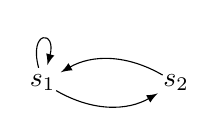
\begin{tikzpicture}[%
        every node/.style={circle,minimum size=4pt,minimum height=4pt, inner sep=0pt},
        shorten >=2pt,
        node distance=1.3cm, >=latex
      ]
      \node [] (0) [circle] {$s_1$};
      \node [] (1) [circle, right=of 0] {$s_2$}; 
      \path [draw] (0) edge[->, bend right]  node {} (1)
      (0) edge[->, loop above]  node {} (0)
      (1) edge[->, bend right]  node {} (0);
    \end{tikzpicture}
    \caption{$M$}
    \label{fig:m}
\end{wrapfigure}

Let $M=(S,I,o_I,T,V,\eqstate{o_1},\eqstate{o_2})$ where $S=I=\{s_1,s_2\}$, $\mathcal{O}=\{o_1,o_2\}$, $o_I=o_1$, $AP=\{q\}$, $o_1$ is the blind observation ($s_1\eqstate{o_1}s_2$) and $o_2$ is the perfect observation ($s\eqstate{o_2}s'\iff s=s')$. $V(s_1)=\{q\}$ and $V(s_2)=\emptyset$. The transitions $T$ are pictured on \textbf{Fig.}~\ref{fig:m}. The augmented model $\hat{M}$ is pictured \textbf{Fig.}~\ref{fig:hatm}. We only drew the reachable states (reachable with $T'$ or $\UD$).

Consider that the formula to model-check is $\varphi=\D{o_2}(\K q\vee\D{o_1}\K\A\X q)$.
Intuitively, it means that if the agent changes to the perfect observation, then either the agent knows that $p$ holds, or even after changing to the blind observation he knows that in every possible next step, $p$ holds.
After running the algorithm, we get the following valuation:

\begin{tabular}{l c l}
$V'(s_1,\{s_1,s_2\},o_1)$ &=& $\{q,p_\varphi\}$\\
$V'(s_2,\{s_1,s_2\},o_1)$ &=& $\{p_\varphi \}$\\
$V'(s_1,\{s_1\},o_1)$ &=& $\{q,p_{(\K q)},p_{(\K q\vee\D{o_1}\K\A\X q)},p_\varphi\}$\\
$V'(s_2,\{s_2\},o_1)$ &=& $\{p_{(\D{o_1}\K\A\X q)},p_{(\K q\vee\D{o_1}\K\A\X q)},p_\varphi\}$\\
$V'(s_1,\{s_1\},o_2)$ &=& $\{q,p_{(\K q)},p_{(\K q\vee\D{o_1}\K\A\X q)},p_\varphi\}$\\
$V'(s_2,\{s_2\},o_2)$ &=& $\{p_{(\D{o_1}\K\A\X q)},p_{(\K q\vee\D{o_1}\K\A\X q)},p_\varphi\}$\\
\end{tabular}

For instance, $q\in V'(s_1,\{s_1\},o_1)$ because $s\in V(s_1)$, $p_{(\K q)}\in V'(s_1,\{s_1\},o_1)$ because $\forall s'\in\{s_1\}, q\in V'(s',\{s_1\},o_1)$.
$p_{(\K q\vee\D{o_1}\K\A\X q)}\in V'(s_1,\{s_1\},o_1)$ because $p_{(\K q)}\in V'(s_1,\{s_1\},o_1)$ and finally, $p_\varphi\in V'(s_1,\{s_1\},o_1)$ because $p_{(\K q\vee\D{o_1}\K\A\X q)}\in V'(s_1,\{s_1\},o_2)$.

We see that $p_\varphi$ is true in every state, and therefore true in the initial states. We conclude, as expected, that $M\models\varphi$.

\begin{figure}
  \centering
    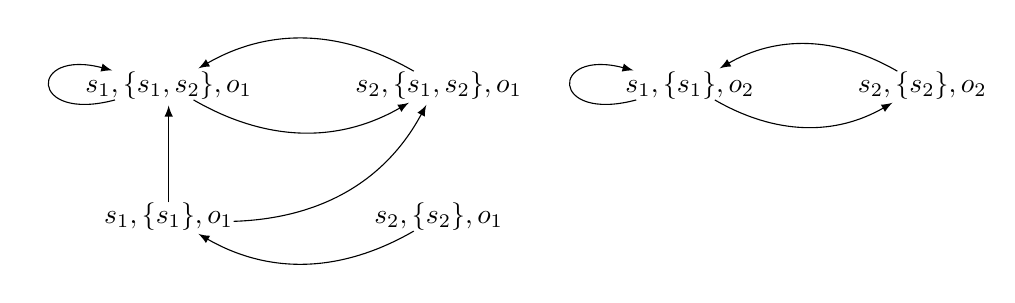
\begin{tikzpicture}[%
        every node/.style={circle,minimum size=4pt,minimum height=4pt, inner sep=0pt},
        shorten >=2pt,
        node distance=1.3cm, >=latex
      ]
      \node [] (0) [rectangle] {$s_1,\{s_1,s_2\},o_1$};
      \node [] (1) [rectangle, right=of 0] {$s_2,\{s_1,s_2\},o_1$};
      \node [] (2) [rectangle, below=of 0] {$s_1,\{s_1\},o_1$};
      \node [] (3) [rectangle, below=of 1] {$s_2,\{s_2\},o_1$};
      \node [] (4) [rectangle, right=of 1] {$s_1,\{s_1\},o_2$};
      \node [] (5) [rectangle, right=of 4] {$s_2,\{s_2\},o_2$};
      \path [draw] (0) edge[->, bend right]  node {} (1)
      (0) edge[->, loop left]  node {} (0)
      (1) edge[->, bend right]  node {} (0)
      (4) edge[->, bend right]  node {} (5)
      (4) edge[->, loop left]  node {} (4)
      (5) edge[->, bend right]  node {} (4)
      (2) edge[->]  node {} (0)
      (2) edge[->, bend right]  node {} (1)
      (3) edge[->, bend left]  node {} (2);
    \end{tikzpicture}
    \caption{$\hat{M}$, the augmented model}
    \label{fig:hatm}
\end{figure}


\section{Multi-agent setting}
\label{sec:multi}
We now define \ctlskd\ for multiple agents.
We consider $\mathcal{A}$ to be the (finite) set of agents. We write $g$ the number of agents.
In this logic, changes of observation are public, meaning that every player knows the changes of observations of all players.
This allows agents to reason about another agent's knowledge.

\subsection{Syntax and intuitive Semantics}
\subsubsection{Syntax}
The syntax has to be modified. There is now one knowledge operator and one change operator for each agent $a\in\mathcal{A}$: $\K_a$ and $\D{o}_a$.

$$\varphi := p ~|~ \neg \varphi ~|~ \varphi\wedge\varphi ~|~ \A\psi ~|~ \K_a\varphi ~|~ \D{o}_a\varphi$$
$$\psi := \varphi ~|~ \neg\psi ~|~ \psi\wedge\psi ~|~ \X\psi ~|~ \psi\U\psi$$

Where $p\in AP, a\in\mathcal{A}$ and $o\in\mathcal{O}$.

\subsubsection{Record Semantics}
We now need one observation record for each player to interpret a formula. For most operators, the semantics remains unchanged. We make the following modifications:

\begin{tabular}{l c l}
$M,h,r_1,\dots,r_g \models\K_a\varphi $&$ \iff $&$ \forall h'$ s.t. $h'\eqh{r_a}h$, we have $M,h',r_1,\dots,r_g\models\varphi$\\
$M,h,r_1,\dots,r_g \models \D{o}_a\varphi$&$ \iff $&$ M,h,r_1,\dots,r_a[(o,|h|-1)],\dots,r_g\models\varphi$
\end{tabular}

\subsection{\ktrees\ semantics}
\subsubsection{\ktrees} We want to define another semantics, similarly to the Information set semantics defined in Section~\ref{sec:alternative}. However, Information sets no longer contain sufficient information to represent the epistemic situation of a multi-agent system. Indeed, agents need not only to remember what states they believe the system might be in, but also the states that other agents believe the system might be in, in case of formulas with nested knowledge operators. For a formula $\phi$ of \ctlskd\ with multiple agent, we write $\mathit{depth}(\phi)$ the maximal number of nested knowledge operators in $\phi$.
For a finite number of nested operators $k$, this information can conveniently be stored in \ktrees, as defined in~\cite{DBLP:conf/fsttcs/MeydenS99}.
The set $\mathcal{T}_k$ of \ktrees\ over the set of states $S$ for $g$ agents is defined inductively as follows:

\begin{tabular}{r l c}
$\mathcal{T}_0$&=&$\{(s,\emptyset,\dots,\emptyset)~|~(g+1)\text{-tuple, with }s\in S\}$\\
$\mathcal{T}_{k+1}$&=&$\{(s,U_1,\dots,U_g)~|~s\in S~\text{ and }\forall i,U_i\subseteq\mathcal{T}_k\}$
\end{tabular}

Intuitively, if $(s,U_1,\dots,U_g)$ is a \ktree, then $s$ (the root) is the real state of the system, and each $U_i$ represents the knowledge of agent $i$. This $U_i$ (the set of $i$-children) is itself a set of $(k-1)$-trees including the knowledge of other agents.

\subsubsection{Updating \ktrees}
Similarly to $\UD$ and $\UT$, we define inductively $\UDK{k}$ and $\UTK{k}$ to update \ktrees.

$\UTK{k}:\mathcal{T}_k\times S\times \mathcal{O}^{g}\rightarrow \mathcal{T}_k$

\begin{center}
$\UTK{0}(t,s,o_1,\dots,o_g) = (s,\emptyset,\dots,\emptyset)$\\
$\UTK{k+1}((s_t,U_{t,1},\dots,U_{t,g}),s,o_1,\dots,o_g)=(s,U_1,\dots,U_g)$\\
$\text{Where }U_i=\{\UTK{k}(t,s',o_1,\dots,o_g)~|~t\in U_{t,i},\quad s'\eqstate{o_i} s,\quad \mathit{root}(t)\ T\ s'\}$
\end{center}

$\UDK{k}:\mathcal{T}_k\times \mathcal{O}^{g}\rightarrow \mathcal{T}_k$

\begin{center}
$\UDK{0}(t,o_1,\dots,o_g)=t$\\
$\UDK{k+1}((s_t,U_{t,1},\dots,U_{t,g}),o_1,\dots,o_g)=(s_t,U_1,\dots,U_g)$\\
$\text{Where }U_i=\{\UDK{k}(t,o_1,\dots,o_g)~|~t\in U_{t,i},\quad\mathit{root}(t)\eqstate{o_i} s_t\}$
\end{center}

Intuitively, when moving to a new state $s$, each agent $i$ has to update his knowledge ($U_i$). The next possible trees will be the update of every tree he considered possible with a state that is equivalent to the new one using the current observation ($o_i$).
When changing observation, we simply remove the trees that are no longer equivalent to the actual state.

\subsubsection{\ktrees\ Semantics}

Let $t=(s,U_1,\dots,U_g)$. We show here the differences with the Information Set semantics:\\
\begin{tabular}{l c l}
  $M,t,o_1,\dots,o_g\models p $&$ \iff $&$ p\in V(\mathit{root}(t))$\\
  $M,t,o_1,\dots,o_g\models\A\psi $&$ \iff $&$ \forall\pi$ such that $\pi_0=\mathit{root}(t)$,\\
  & & we have $M,\pi,t,o_1,\dots,o_g\models\psi$\\
  $M,t,o_1,\dots,o_g\models\K_i\varphi $&$ \iff $&$ \forall t'\in U_i$, we have $M,t',o_1,\dots,o_g\models\varphi$\\
  $M,t,o_1,\dots,o_g'\models\D{o'}_i\varphi $&$ \iff $&$ M,\UD(t,o_1,\dots,o',\dots,o_g),o_1,\dots,o',\dots,o_g\models\varphi$\\
  $M,\pi,t,o_1,\dots,o_g\models\varphi $&$ \iff $&$ M,t,o_1,\dots,o_g\models\varphi$\\
  $M,\pi,t,o_1,\dots,o_g\models\X\psi $&$ \iff $&$ M,\pi_{1\dots},\UT(t,\pi_1,o_1,\dots,o_g),o_1,\dots,o_g\models\psi$\\
  $M,\pi,t,o_1,\dots,o_g\models\psi_1\U\psi_2 $&$ \iff $&$ \exists n\geq 0$, $\forall m\leq n,$\\
  & & $M,\pi_{m\dots},\UT^m(t,\pi,o_1,\dots,o_g),o_1,\dots,o_g\models\psi_1$\\
  & & and $M,\pi_{n\dots},\UT^n(t,\pi,o_1,\dots,o_g),o_1,\dots,o_g\models\psi_2$
\end{tabular}

An adaptation of the reduction theorem can be found in Section~\ref{subsec:reduc}. The modified model-checking algorithm can be found in Section~\ref{subsec:mc}. Now that we successfully defined the data structure that holds the epistemic information and how to update it, the way to model-checking is similar to the single-agent setting, with \ktrees\ instead of information sets.


\section{Conclusion and Future Works}
\label{sec:conclusion}
\begin{frame}{Multi agent setting}
  \begin{block}{New syntax}
    \begin{tabular}{r l}
    History Formula: & $\varphi := p ~|~ \neg \varphi ~|~ \varphi\wedge\varphi ~|~ \A\psi ~|~ \K_a\varphi ~|~ \D{o}_a\varphi$\\
    Path Formula: & $\psi := \varphi ~|~ \neg\psi ~|~ \psi\wedge\psi ~|~ \X\psi ~|~ \psi\U\psi$
    \end{tabular}
    
    $a$ agent.
  \end{block}
  \vfill
  \begin{block}{\ktrees}
    \begin{center}
      \begin{tikzpicture}[%
      every node/.style={circle,minimum size=4pt,minimum height=4pt, inner sep=0pt},
      shorten >=2pt,
      node distance=1.3cm, >=latex
    ]
        \node [] (0) [circle] {$s_1$};
        \node [] (4) [circle, below left=of 0,xshift=-2cm] {,};
    \node [] (1) [circle, left=of 4,xshift=1cm] {$\{~s_1$};
    \node [] (2) [circle, right=of 4,xshift=-1cm] {$s_2~\}$};
    \node [] (3) [circle, below right=of 0,xshift=2cm] {$\{\quad s_1\quad\}$};
    \node [] (11) [circle, below left=of 1] {$\{s_1\}$};
    \node [] (12) [circle, below=of 1] {$\{s_1\}$};11
    \node [] (21) [circle, below=of 2] {$\{s_2\}$};
    \node [] (22) [circle, below right=of 2] {$\{s_2\}$};    
    \node [] (31) [circle, below left=of 3] {$\{s_1,s_2\}$};
    \node [] (32) [circle, below right=of 3] {$\{s_1\}$};    

    \path
    (0) edge[->,above left]  node {\tiny 1} (4)
    (0) edge[->,above right]  node {\tiny 2} (3)
    (1) edge[->,above left] node {\tiny 1} (11)
    (1) edge[->,right] node {\tiny 2} (12)
    (2) edge[->,left] node {\tiny 1} (21)
    (2) edge[->,above right] node {\tiny 2} (22)
    (3) edge[->,above left] node {\tiny 1} (31)
    (3) edge[->,above right] node {\tiny 2} (32)
    ;
      \end{tikzpicture}
    \end{center}
  \end{block}

\end{frame}


\begin{frame}{Summary}

  \begin{exampleblock}{Definition of \ctlskd}
    First one to study changes of observations with epistemic operators.
  \end{exampleblock}
  \vfill
  \begin{exampleblock}{Definition of alternative semantics}
    Easier to model-check.\\
    Proved the equivalence between the two semantics.
  \end{exampleblock}
  \vfill
  \begin{exampleblock}{Model-Checking}
    Marking Algorithm.\\
    EXPTIME for single-agent setting.
  \end{exampleblock}
  \vfill
  \begin{exampleblock}{Multi-agent setting}
    Nonelementary complexity for model-checking.
  \end{exampleblock}
   
\end{frame}


\begin{frame}{Future Works}

  \begin{itemize}
  \item Extend the logic. Allow $\D{o}$ in path formulas.
  \item Axiomatization of \ctlskd.
  \item Implementation of the Model-Checking Algorithm.
  \item Epistemic Extension of Strategy Logic with Imperfect Information.
  \end{itemize}
  
\end{frame}


\newpage
\pagenumbering{Roman}
%\nocite{*}
\bibliographystyle{plain}
\bibliography{../bib/slii.bib}

\newpage
\section{Appendix}
\subsection{Lemmas Proofs}
\label{subsec:lemmaproof}

\paragraph{Lemma 1}
Let $h,h'$ and $r$ such that $h\eqh{r}h'$. Let $(s,I,o)=\FV(h,r)$ and $(s',I',o')=\FV(h',r)$. We have $I=I'$ and $o=o'$.\\
\textbf{Proof:} $I=I'$ according to the \textbf{Information Set Lemma}. In \textsc{ii)}, we see that the observation only depends on the record and the length of the history. $|h|=|h'|$ because $h\eqh{r}h'$ and thus $o=o'$.\qed

\paragraph{Lemma 2}
Let $(s,I,o)=\FV(h,r)$. Then, $\forall\pi$ such that $\pi_0=s$, $\FP(h.\pi_{1\dots},|h|-1,r)=(\pi,I,o)$.\\
\textbf{Proof:} \begin{itemize}
\item\textsc{iv)} $(h.\pi_{1\dots})_n=s=\pi_0$ and $\forall i\in\mathbb{N}, (h.\pi_{1\dots})_{n+i}=\pi_i$.
\item\textsc{v)} $o=\mathit{last}(r_{\leq |h|-1})$ because $(s,I,o)=\FV(h,r)$ (\textsc{ii}).
\item\textsc{vi)} Because $(s,I,o)=\FV(h,r)$ (\textsc{iii}).\qed
\end{itemize}

\paragraph{Lemma 3}
Let $(s,I,o)=\FV(h,r)$. Then, $\FV(h,r[(o',|h|-1)])=(s,\UD(I,s,o'),o')$.\\
\textbf{Proof:} \begin{itemize}
\item\textsc{i)} Because $(s,I,o)=\FV(h,r)$ (\textsc{I}).
\item\textsc{ii)} Because $o'=\mathit{last}(r[(o',|h|-1)]_{\leq |h|-1})$.
\item\textsc{iii)} We have $f(h,r[(o',|h|-1)])=\UD(f(h,r),\mathit{last(h)},o')$. Because $(s,I,o)=\FV(h,r)$ (\textsc{iii}), $f(h,r)=I$ and (\textsc{i}) $\mathit{last}(h)=s$. Thus, $f(h,r[(o',|h|-1)])=\UD(I,s,o')$.\qed
\end{itemize}

\paragraph{Lemma 4}
Let $(\pi',I,o)=\FP(\pi,n,r)$. Then, $\FV(\pi_0\dots\pi_n,r)=(\pi'_0,I,o)$.\\
\textbf{Proof:} \begin{itemize}
\item\textsc{i)} $\pi'_0=\pi_n$ because $(\pi',I,o)=\FP(\pi,n,r)$ (\textsc{iv}).
\item\textsc{ii)} Because $(\pi',I,o)=\FP(\pi,n,r)$ (\textsc{v}).
\item\textsc{iii)} Because $(\pi',I,o)=\FP(\pi,n,r)$ (\textsc{vi}).\qed
\end{itemize}

\paragraph{Lemma 5}
Let $(\pi',I,o)=\FP(\pi,n,r)$. Then, $\FP(\pi,n+1,r)=(\pi'_{1\dots},\UT(I,\pi'_1,o),o)$.\\
\textbf{Proof:}
First, $\FP(\pi,n+1,r)$ is defined because $r=r_{\leq n}=r_{\leq n+1}$.
\begin{itemize}
\item\textsc{iv)} Because $(\pi',I,o)=\FP(\pi,n,r)$ (\textsc{iv}), $\pi'=\pi_{n\dots}$ and thus $\pi'_{1\dots}=\pi_{n+1\dots}$.
\item\textsc{v)} Because $(\pi',I,o)=\FP(\pi,n,r)$ (\textsc{v}).
\item\textsc{vi)} We have $f((\pi_0\dots\pi_{n+1}),r_{\leq n})=\UT(f(\pi_0\dots\pi_n,r_{\leq n}),\pi_{n+1},o)$. Because $(\pi',I,o)=\FP(\pi,n,r)$ (\textsc{vi}), we have $f(\pi_0\dots\pi_n,r_{\leq n})=I$. Thus, $f((\pi_0\dots\pi_{n+1}),r_{\leq n})=\UT(I,\pi'_1,o)$.\qed
\end{itemize}

\paragraph{Lemma 6}
Let $(\pi',I,o)=\FP(\pi,n,r)$. Then, $\forall k\geq 0, \FP(\pi,n+k,r)=(\pi'_{k\dots},\UT^k(I,\pi',o),o)$.\\
\textbf{Proof} We proceed by induction.
For $k=0$, we have to prove $(\pi'_{0\dots},I,o)=\FP(\pi,n+0,r)$, which is our hypothesis.
For the inductive case:
\begin{itemize}
\item\textsc{iv)} $\pi_{n+k\dots}=\pi'_{k\dots}$ because $(\pi',I,o)=\FP(\pi,n,r)$ (\textsc{iv}).
\item\textsc{v)}  Because $(\pi',I,o)=\FP(\pi,n,r)$ (\textsc{v}) and $r=r_{\leq n}$.
\item\textsc{vi)} By induction hypothesis, $f(\pi_0\dots\pi_{n+k},r)=\UT^k(I,\pi',o)$. Then, $f(\pi_0\dots\pi_{n+k+1},r)=\UT(\UT^k(I,\pi',o),\pi_{n+k=1},o)=\UT^{k+1}(I,\pi',o)$ because $r_{n+k+1}$ is empty.\qed
\end{itemize}

\subsection{Reduction Theorem for multiple agents}
\label{subsec:reduc}
From $k\in\mathbb{N}$, a history $h$ and observation record $r_1,\dots,r_g$, we can get a corresponding \ktree\ and current observations. Similarly, from $k$, an infinite sequence $\pi$, a time $n$ and records, we can get corresponding sequence $\pi'$ that starts at the current state, \ktree\ and current observations.

We can define two partial functions, $\FV$ and $\FP$, similarly to what was done for the single agent setting, Section~\ref{sec:alternative}:
$\FV(k,h,r_1,\dots,r_g)=(t,o_1,\dots,o_g)$ and 
$\FP(k,\pi,n,r_1,\dots,r_g)=(\pi',t,o_1,\dots,o_g)$.

Finally, the Reduction Theorem can be adapted as follows:\\
$\forall\phi$ formula of \ctlskd, $k=\mathit{depth}(\phi)$,\\
if $\phi=\varphi$ is a history formula, $\forall h,r_1,\dots,r_g,t,o_1,\dots,o_g$ such that $\FV(k,h,r_1,\dots,r_g)=(t,o_1,\dots,o_g)$, \quad$M,k,h,r_1,\dots,r_g\models\varphi\iff M,t,o_1,\dots,o_g\models\varphi$,\\
if $\phi=\psi$ is a path formula, $\forall \pi,n,r_1,\dots,r_g,\pi',t,o_1,\dots,o_g$ such that $\FP(k,\pi,n,r_1,\dots,r_g)=(\pi',t,o_1,\dots,o_g)$, \quad$M,\pi,n,r_1,\dots,r_g\models\psi\iff M,\pi',t,o_1,\dots,o_g\models\psi$.

\subsection{Model-Checking a \ctlskd\ formula for multiple agents}
\label{subsec:mc}
The new extended model is the following: $\hat{M}=(S'_1\cup\dots\cup S'_{\mathit{depth}(\varphi)},T',V')$.
\begin{itemize}
\item $\forall i, S'_i=\mathcal{T}_i\times \mathcal{O}^g$: states are an $i$-tree and an observation for each player.
\item $(t,o_1,\dots,o_g)~T'~(t',o_1,\dots,o_g)\iff \mathit{root}(t)~T~\mathit{root}(t')$ and $t'=\UTK{i}(t,\mathit{root}(t'),o_1,\dots,o_g)$
\item $V'(t,o_1,\dots,o_g)=V(\mathit{root}(t))$. As the algorithm is executed, new atomic propositions will appear. We will update $V'$ accordingly.
\end{itemize}
The algorithm is a marking algorithm very similar to what has been described in Section~\ref{sec:mc}. For each $\K_i\varphi$ or $\D{o}_i\varphi$ formula where $\varphi$ is a \ctls\ formula, we first check $\varphi$ on each state. Then, we mark $(t,o_1,\dots,o_g)$ with $p_{\K_i\varphi}$ if $t\in\mathcal{T}_k$ with $k\geq\mathit{depth}(\K\varphi)$ and $\forall t'$ $i$-child of $t$, $(t',o_1,\dots,o_g)$ has been marked by $p_\varphi$. We mark it with $p_{\D{o'}_i\varphi}$ if $(t,o_1,\dots,o_{i-1},o',\dots,o_g)$ has been marked with $p_\varphi$.

The number of \ktrees\ has been studied in~\cite{DBLP:conf/fsttcs/MeydenS99}. Our model-checking algorithm for multiple agents has non-elementary complexity.


\end{document}
